\documentclass[11pt,a4paper]{article}

% ---------------------------------------------------------------------------
% Collective thermodynamic incompatibility of autocatalytic cores:
% minimally incompatible families of unbounded order.
%
% Author metadata: set the three macros below before submission.
% ---------------------------------------------------------------------------
\newcommand{\PaperAuthor}{Anonymous manuscript}
\newcommand{\PaperAffiliation}{}
\newcommand{\PaperDate}{September 13, 2026}

\usepackage[T1]{fontenc}
\usepackage[utf8]{inputenc}
\usepackage{lmodern}
\usepackage{microtype}
\usepackage[a4paper,margin=1.05in]{geometry}
\usepackage{amsmath,amssymb,amsthm,mathtools}
\usepackage{booktabs}
\usepackage{array}
\usepackage{enumitem}
\usepackage{xcolor}
\usepackage{graphicx}
\usepackage{tikz}
\usetikzlibrary{arrows.meta,positioning,calc}
\usepackage{listings}
\usepackage[obeyspaces,spaces]{url}
\usepackage[numbers,sort&compress]{natbib}
\usepackage[colorlinks=true,linkcolor=blue!55!black,citecolor=blue!55!black,urlcolor=blue!55!black]{hyperref}

\setlist{itemsep=2pt,topsep=3pt}
\setlength{\emergencystretch}{1.5em}

\theoremstyle{plain}
\newtheorem{theorem}{Theorem}[section]
\newtheorem{proposition}[theorem]{Proposition}
\newtheorem{lemma}[theorem]{Lemma}
\newtheorem{corollary}[theorem]{Corollary}
\theoremstyle{definition}
\newtheorem{definition}[theorem]{Definition}
\newtheorem{construction}[theorem]{Construction}
\newtheorem{example}[theorem]{Example}
\theoremstyle{remark}
\newtheorem{remark}[theorem]{Remark}

\lstdefinelanguage{Lean}{
  morekeywords={theorem,def,structure,inductive,namespace,end,import,by,intro,exact,constructor,refine,where,abbrev,noncomputable,rintro,simpa,using},
  sensitive=true,
  morecomment=[l]{--},
  morestring=[b]",
}
\lstset{
  language=Lean,
  basicstyle=\ttfamily\small,
  keywordstyle=\bfseries,
  commentstyle=\itshape\color{black!60},
  columns=fullflexible,
  keepspaces=true,
  breaklines=true,
  frame=single,
  framerule=0.3pt,
  xleftmargin=1em,
  xrightmargin=1em,
  extendedchars=true,
  literate={≤}{{$\le$}}1 {≥}{{$\ge$}}1 {ℕ}{{$\mathbb{N}$}}1 {ℝ}{{$\mathbb{R}$}}1 {→}{{$\to$}}1 {∀}{{$\forall$}}1 {∃}{{$\exists$}}1 {≠}{{$\neq$}}1 {∧}{{$\wedge$}}1 {¬}{{$\neg$}}1 {↔}{{$\leftrightarrow$}}1 {∑}{{$\sum$}}1 {∏}{{$\prod$}}1 {₀}{{$_0$}}1 {₁}{{$_1$}}1 {₂}{{$_2$}}1 {⟨}{{$\langle$}}1 {⟩}{{$\rangle$}}1 {∈}{{$\in$}}1 {·}{{$\cdot$}}1 {α}{{$\alpha$}}1 {β}{{$\beta$}}1 {μ}{{$\mu$}}1 {ι}{{$\iota$}}1
}

\newcommand{\R}{\mathbb{R}}
\newcommand{\N}{\mathbb{N}}
\newcommand{\Z}{\mathbb{Z}}
\newcommand{\Rpos}{\R_{>0}}
\newcommand{\cS}{\mathcal{S}}
\newcommand{\cR}{\mathcal{R}}
\newcommand{\cE}{\mathcal{E}}
\newcommand{\cF}{\mathcal{F}}
\newcommand{\cH}{\mathcal{H}}
\newcommand{\Comp}{\mathsf{Comp}}
\newcommand{\DIR}{\mathsf{Dir}}
\newcommand{\LIN}{\mathsf{LinCx}}
\DeclareUrlCommand\lean{\urlstyle{tt}}   % breaks at . and _ ; write underscores unescaped inside \lean{}
\newcommand{\hash}[1]{\texttt{\scriptsize #1}}
\newcommand{\rev}{\rightleftharpoons}
\DeclareMathOperator{\rank}{rk}

\title{Collective thermodynamic incompatibility of autocatalytic cores:\\ minimally incompatible families of unbounded order}
\author{\PaperAuthor\\ \PaperAffiliation}
\date{\PaperDate}

\begin{document}
\maketitle

\begin{abstract}
A potential autocatalytic core (PAC) is a minimal stoichiometric motif admitting a strictly productive reaction current. Kosc, Kuperberg, Rajon and Charlat (\emph{Proc.\ Natl.\ Acad.\ Sci.\ USA}, 2025) proved that every isolated PAC can be realized by a positive activity vector under thermodynamically consistent mass action, and showed that families of interacting cores need not be jointly realizable; our predecessor paper quantified the two-core case exactly. Here we study the \emph{order} of a collective conflict. Fix a reversible network with fixed transition-state factors and an activity box, call a family of selected cores compatible if one activity vector makes every selected core productive with its reactions running in the displayed directions, and call a family minimally incompatible if it is incompatible while every proper subfamily is compatible. We prove that minimally incompatible families of every order $n\ge 3$ exist among the sparsest conceivable cores: $n$ unit-factor two-reaction cores $X_s\rev X_t$, $X_t\rev 2X_s$ on $n$ species, arranged as a directed path with one shortcut. The full family has no common productive state anywhere in the positive orthant, every proper subfamily has one in $[9/10,1]^n$, and the full family nevertheless passes both standard necessary relaxations, reaction-direction feasibility and independent-complex feasibility, with witnesses inside the same box. The obstruction is a single exact inequality $f(f(x))<g(x)$ between a two-step response and the shortcut response. Consequently no test based on subfamilies of bounded size, even combined with both global relaxations, decides compatibility. Complementing this, we give an exact univariate elimination theorem for arbitrary bounded fans of autocatalytic triangles sharing one reaction; a three-triangle fan that is minimally incompatible on an explicit open neighbourhood of all seven kinetic factors and ten box endpoints while passing both relaxations; and a polynomial-time constructive compatibility certificate for graded assemblies of two-reaction cores. All source-level statements are verified in Lean~4 against Mathlib, and the hand-proved complements are listed explicitly.
\end{abstract}

\noindent\textbf{Keywords.} autocatalysis; autocatalytic cores; chemical reaction networks; mass-action kinetics; thermodynamic consistency; minimal infeasible subsystems; Helly-type bounds; formal verification.

\medskip
\noindent\textbf{MSC 2020.} 92E20, 80A30, 90C05, 52A35, 68V20.

\section{Introduction}\label{sec:intro}

Autocatalysis, the capacity of a set of species to catalyse its own net production, is a basic ingredient of scenarios for the emergence of Darwinian dynamics in chemistry \citep{blokhuis2020,hordijk2004,steel2020}. Blokhuis, Lacoste and Nghe \citep{blokhuis2020} made the notion stoichiometric: a motif of a reaction network is autocatalytic when some reaction current strictly increases every one of its species, and the minimal such motifs are the \emph{autocatalytic cores}. Cores are combinatorial objects and know nothing about rate constants or free energies. Kosc, Kuperberg, Rajon and Charlat \citep{kosc2025} asked whether a stoichiometrically autocatalytic motif can actually run under thermodynamically consistent kinetics, and proved a striking positive answer for a single core: every potential autocatalytic core (PAC) is a consistent autocatalytic core, that is, for any transition-state factors some positive activity vector drives its productive current. They also observed that this realizability does not survive interaction: two cores that share reactions may admit a common productive current and still admit no common activity vector.

Our predecessor paper \citep{tcic2026} studied that failure for two cores. It refuted the natural strengthening of the isolated-core theorem, in which a common productive current and a common direction potential are asked to imply a common realization; it proved an exact phase diagram for two autocatalytic triangles with a shared reaction, $1/2<k<2$ in the ratio $k$ of private factors; it derived an exact scalar interface interval for eliminating a triangle; and it separated three logically distinct obstruction layers, reaction direction, barrier-weighted magnitude, and the monomial lift from complex activities to species activities.

This paper asks a question that only makes sense for more than two cores. Compatibility of a family of cores is downward closed: whatever a common state does for a family, it does for every subfamily. It is therefore natural to organize incompatibility by its \emph{minimal} witnesses, the families that are incompatible while every proper subfamily is compatible, and to ask how large such a minimal conflict can be. If the minimal conflicts of a class of networks had bounded order $k$, compatibility of every family in the class would be certified by checking its subfamilies of size at most $k$, a local test in the spirit of Helly's theorem \citep{helly1923,eckhoff1993} for convex sets. If in addition the two global necessary relaxations used in the predecessor, direction feasibility and independent-complex feasibility, were adjoined to such a local test, one might hope for a complete finite procedure.

We show that no such bounded order exists, even for cores that are as small and sparse as possible, and even when both global relaxations are adjoined. The construction is transparent: $n$ two-reaction cores $X_s\rev X_t$, $X_t\rev 2X_s$ on $n$ species, arranged as a directed path $0\to1\to\dots\to L$ with the single shortcut $0\to L$, $n=L+1\ge3$. Productivity of one such core with source activity $x$ pins the target activity $y$ into the exact open interval $g(x)<y<f(x)$ with $f(x)=(x+x^2)/2$ and $g(x)=(x+2x^2)/3$, and the whole phenomenon rests on the identity
\[
f(f(x))-g(x)=\frac{x(x-1)(3x^2+9x+2)}{24}<0\qquad(0<x<1):
\]
two steps along the path push the activity strictly below what the shortcut demands. Deleting any one core restores a common state by an explicit rank-graded formula, and the full family still admits a bounded state with all $2n$ reactions running in their displayed directions, together with a single global assignment of independent complex activities that makes every core productive.

\subsection{Main results}\label{sec:mainresults}

We work with a finite reversible network $Q$ in which reaction $r$ has reactant complex $\alpha_r$, product complex $\beta_r$ and a positive transition-state factor $b_r$; for a positive activity vector $z$ the oriented current is $j_r(z)=b_r(z^{\alpha_r}-z^{\beta_r})$, the model of \citep{kosc2025} and \citep{tcic2026}. A \emph{selected family} is a finite family of PACs of $Q$ with a displayed orientation of every reaction it uses, together with a fixed activity domain $\Omega$. A subfamily is \emph{compatible} if one $z\in\Omega$ makes each of its cores productive with each of its reactions running forward; deleting a core removes only that core's requirements, and leaves factors, boxes and the currents of shared reactions untouched (Section~\ref{sec:setting}). Our results are as follows; each is stated informally here and precisely in the body of the paper.

\begin{enumerate}[label=(\Alph*)]
\item\label{res:A} \textbf{Minimal conflicts of every order (Theorem~\ref{thm:order}).} For every $n\ge3$ there is a selected family of $n$ two-reaction PACs on $n$ species, with unit factors and complexes of molecularity at most two, that is incompatible on the whole positive orthant, whose every proper subfamily is compatible inside $[9/10,1]^n$, and that passes direction feasibility and independent-complex feasibility with witnesses inside the same box. Consequently (Corollary~\ref{cor:local}) no test of bounded subfamily order, even supplemented by both relaxations, is sufficient for compatibility.
\item\label{res:B} \textbf{Exact fan elimination (Theorem~\ref{thm:fan}).} For any finite fan of autocatalytic triangles $A\rev B\rev C_i\rev m_iA$ sharing the reaction $A\rev B$, with arbitrary positive factors and closed positive boxes on every species, compatibility is equivalent to the existence of one shared activity $a$ in its box satisfying an explicit finite system of strict polynomial comparisons; private activities and the shared $B$ are eliminated exactly and reconstructed explicitly.
\item\label{res:C} \textbf{A robust minimal triple (Theorem~\ref{thm:robust}).} A specific three-triangle fan with gains $(3,4,3)$ is minimally incompatible, passes both relaxations, and remains minimally incompatible when all seven kinetic factors and all ten box endpoints are perturbed independently by up to $10^{-6}$; a two-parameter window of private box endpoints is also covered exactly (Proposition~\ref{prop:window}). The obstruction is a monomial-layer one: it disappears as soon as $A^3$ and $A^4$ are allowed to be independent variables.
\item\label{res:D} \textbf{Graded assemblies (Theorems~\ref{thm:graded} and~\ref{thm:recognition}).} Any assembly of two-reaction cores whose species admit integer ranks increasing by one along every core has an explicit common rational state, and this graded class is recognizable, with the state constructed, in polynomial time. Acyclicity alone does not suffice, by~\ref{res:A}.
\item\label{res:E} \textbf{Formal verification (Section~\ref{sec:formal}).} The source-level statements behind~\ref{res:A}--\ref{res:D}, including PAC minimality of every core involved under signed flows, are compiled in Lean~4 \citep{demoura2021} against Mathlib \citep{mathlib2020} with warnings treated as errors and no admitted statements. The conventional complements (channel counting, the algorithmic complexity bound, the persistence of the relaxation witnesses in the perturbation cube, and the chemical food interpretation) are listed in Section~\ref{sec:notformal}.
\end{enumerate}

The three obstruction layers of the predecessor reappear here at every order. The ring of $n$ two-reaction cores around a cycle (Proposition~\ref{prop:ring}) is a minimal conflict of order $n$ that already fails direction feasibility; the path with a shortcut is a minimal conflict of order $n$ that passes both direction and independent-complex feasibility and fails only at the monomial lift; and the fan triple of~\ref{res:C} is a three-core magnitude-and-lift conflict that persists on an open set of parameters. In each case the number of species grows with the order, so no dimension-dependent Helly theorem is contradicted (Remark~\ref{rem:helly}).

\subsection{Relation to previous work}

The framework of stoichiometric autocatalytic cores is due to Blokhuis, Lacoste and Nghe \citep{blokhuis2020}; its diluted-regime dynamics were developed by Unterberger and Nghe \citep{unterberger2022} and Nandan, Nghe and Unterberger \citep{nandan2025}, and cores with explicit catalysis are treated by Golnik, Gatter, Stadler and Vassena \citep{golnik2026cores}. The thermodynamic realizability question and the PAC/CAC distinction are from Kosc et al.\ \citep{kosc2025}, whose isolated-core theorem and interacting counterexample are the starting point of \citep{tcic2026} and of this paper. The polyhedral geometry of autocatalytic subnetworks is studied in \citep{gagrani2024}; recognizing autocatalysis is NP-complete \citep{andersen2012,kosc2025}. Vassena and Stadler \citep{vassena2024} concern dynamical instability, a question orthogonal to the existence of a static witness studied here. Despons, De Decker and Lacoste \citep{despons2024} bound affinities at optimal flux, a different regime.

That stoichiometric feasibility does not imply thermodynamic feasibility is classical in metabolic network analysis: energy-balance analysis \citep{beard2002} and the loop-law constraints of \citep{beard2004} exclude flux distributions that violate the second law. Those constraints are direction-level: they concern signs of affinities and are equivalent to our direction relaxation. The content of the present paper is that, for autocatalytic cores with fixed transition-state factors, the direction level and even the independent-complex level are far from sufficient, and that the residual nonlinear coupling supports minimal conflicts of unbounded order. The phrase ``compatibility hypergraph'' is our name for the family of minimal conflicts; it is not attributed to prior literature, and the bounded novelty audit reported in \citep{tcic2026} is not a proof of absence.

\subsection{Organization}

Section~\ref{sec:setting} fixes the model, the selected-subfamily semantics and the two relaxations. Section~\ref{sec:pairs} develops the response calculus of two-reaction cores. Section~\ref{sec:order} proves the unbounded-order theorem, with a worked instance, the local-testing corollary and the direction-layer ring. Section~\ref{sec:fan} proves exact fan elimination, Section~\ref{sec:robust} the robust triple, and Section~\ref{sec:graded} the graded class and its recognition. Section~\ref{sec:chemistry} discusses chemical interpretation and scope, Section~\ref{sec:formal} documents the formal verification, and Section~\ref{sec:discussion} concludes.

\section{Setting}\label{sec:setting}

\subsection{Reversible networks and currents}

\begin{definition}[Reversible network]\label{def:crn}
A \emph{reversible network} $Q=(\cS,\cR,\alpha,\beta,b)$ consists of finite sets $\cS$ of species and $\cR$ of reactions, reactant and product complexes $\alpha_r,\beta_r\in\N^{\cS}$ for each $r\in\cR$, and positive factors $b_r>0$. The stoichiometric coefficient of $s$ in $r$ is $\beta_{rs}-\alpha_{rs}$. For $z\in\Rpos^{\cS}$ and a complex $c$ write $z^{c}=\prod_s z_s^{c_s}$. The \emph{current} of $r$ at $z$ is
\[
j_r(z)=b_r\bigl(z^{\alpha_r}-z^{\beta_r}\bigr).
\]
\end{definition}

Physically, $z_s=e^{\mu_s/RT}$ is an activity and $b_r$ is a transition-state factor \citep{eyring1935,kosc2025}; the same $b_r$ multiplies both directions, so the equilibrium ratio is fixed by the endpoint free energies. All statements below are about existence of a positive static witness; no steady-state, dilute-regime or tight-coupling assumption is used.

\subsection{Motifs and potential autocatalytic cores}

\begin{definition}[Motifs, productivity, PAC]\label{def:motif}
A \emph{motif} $C=(\cS_C,\cR_C)$ of $Q$ is a pair of subsets $\cS_C\subseteq\cS$, $\cR_C\subseteq\cR$. It is \emph{side-incident} if both sets are nonempty and every $r\in\cR_C$ has a species of $\cS_C$ with positive coefficient in $\alpha_r$ and one with positive coefficient in $\beta_r$. For a flow $v\in\R^{\cR}$, the \emph{production residual} of $C$ at $s\in\cS_C$ is $\sum_{r\in\cR_C}(\beta_{rs}-\alpha_{rs})v_r$, and $C$ is \emph{productive} for $v$ if every residual is strictly positive. $C$ is an \emph{autocatalytic motif} if it is side-incident and productive for some $v\in\R^{\cR}$, and a \emph{potential autocatalytic core} (PAC) if it is an autocatalytic motif and no strict submotif (a motif with $\cS_{C'}\subseteq\cS_C$, $\cR_{C'}\subseteq\cR_C$ and at least one inclusion strict) is an autocatalytic motif.
\end{definition}

Minimality is tested against arbitrary \emph{signed} flows of the submotif, not only against flows in a prescribed positive orientation; this is the source-faithful reading of \citep{kosc2025} adopted in \citep{tcic2026}, and it is the notion checked formally for every core in this paper.

\subsection{Selected families and the compatibility predicate}

\begin{definition}[Selected family, compatibility]\label{def:family}
A \emph{selected family} on $Q$ is a finite indexed family $(C_i)_{i\in\cE}$ of PACs of $Q$, each reaction used by some $C_i$ carrying a displayed orientation (in this paper every reaction is displayed in the direction in which it is written), together with an \emph{activity domain} $\Omega\subseteq\Rpos^{\cS}$. For $F\subseteq\cE$ the predicate $\Comp_\Omega(F)$ holds if there is $z\in\Omega$ such that for every $i\in F$ the motif $C_i$ is productive for the current $j(z)$ and $j_r(z)>0$ for every $r\in\cR_{C_i}$.
\end{definition}

Three features of this predicate matter. First, a shared reaction has one current $j_r(z)$ wherever it occurs; there is no independent copy per core. Second, deleting a core from $F$ removes only that core's production and direction requirements; the domain $\Omega$, all factors, and all species (including the deleted core's private species, which must still take a value in $\Omega$) remain in place. Third, an omitted core's reactions are neither removed from the network nor forced to carry zero current. This is the \emph{selected-subfamily} predicate; it differs from a whole-network predicate that would retain the directions of omitted cores, and the distinction is decisive for every deletion argument below.

\begin{lemma}[Downward closure]\label{lem:down}
If $F\subseteq G\subseteq\cE$ and $\Comp_\Omega(G)$, then $\Comp_\Omega(F)$.
\end{lemma}
\begin{proof}
The witness for $G$ satisfies the requirements of every $i\in F$.
\end{proof}

\begin{definition}[Minimal conflicts]\label{def:minimal}
$F\subseteq\cE$ is \emph{minimally incompatible} if $\neg\Comp_\Omega(F)$ and $\Comp_\Omega(F\setminus\{i\})$ for every $i\in F$. By Lemma~\ref{lem:down} every proper subfamily of a minimally incompatible family is then compatible. The set $\cH_{\Omega}$ of minimally incompatible subfamilies is the \emph{conflict hypergraph} of the selected family; its \emph{order} is the size of a hyperedge.
\end{definition}

The conflict hypergraph records the selected-family predicate; it does not assert that the selected cores exhaust the PACs of $Q$, and it does not concern core detection.

\subsection{Two necessary relaxations}

\begin{definition}[Direction and independent-complex feasibility]\label{def:relax}
Let $F\subseteq\cE$ and let $\cR_F$ be the set of reactions used by cores of $F$.
\begin{itemize}
\item \emph{Direction feasibility} $\DIR_\Omega(F)$: some $z\in\Omega$ has $j_r(z)>0$ for all $r\in\cR_F$.
\item \emph{Independent-complex feasibility} $\LIN(F)$: some assignment $y$ of a positive number $y_c$ to every distinct complex $c$ occurring in $\cR_F$, shared by all occurrences of $c$, makes the linear currents $\tilde\jmath_r=b_r(y_{\alpha_r}-y_{\beta_r})$ positive for all $r\in\cR_F$ and every $C_i$, $i\in F$, productive for $\tilde\jmath$.
\end{itemize}
Bounds on individual complex values, when claimed, are additional requirements.
\end{definition}

\begin{lemma}[Necessity]\label{lem:necessary}
$\Comp_\Omega(F)$ implies $\DIR_\Omega(F)$ and $\LIN(F)$. For $\Omega=\Rpos^{\cS}$, $\DIR_\Omega(F)$ holds if and only if some potential $\mu\in\R^{\cS}$ has $\langle\alpha_r-\beta_r,\mu\rangle>0$ for all $r\in\cR_F$.
\end{lemma}
\begin{proof}
A compatible witness $z$ is a direction witness, and $y_c=z^c$ is an independent-complex witness because $\tilde\jmath_r=j_r(z)$. For the second claim put $z=e^{\mu}$ coordinatewise: $j_r(z)>0$ if and only if $\langle\alpha_r,\mu\rangle>\langle\beta_r,\mu\rangle$.
\end{proof}

Thus $\DIR$ on the orthant is the direction-potential predicate of \citep{tcic2026} and the loop-law feasibility of \citep{beard2004}; on a box it is stronger. $\LIN$ retains the barrier-weighted magnitudes of the currents but forgets that $y_c$ must be the monomial $z^c$ of a single species vector; it is the linear-complex predicate of \citep{tcic2026}. Neither relaxation requires the equations $y_c=z^c$ that couple different complexes, and Theorem~\ref{thm:order} shows that precisely this coupling supports conflicts of every order.

\section{Two-reaction cores and their response calculus}\label{sec:pairs}

The building block of Sections~\ref{sec:order} and~\ref{sec:graded} is the smallest reversible autocatalytic motif with a gain of two. For species $X_s\neq X_t$ the \emph{pair} $P(s,t)$ consists of the two reactions
\begin{equation}\label{eq:pair}
X_s\rev X_t,\qquad X_t\rev 2X_s,
\end{equation}
both with factor one, on the species $\{X_s,X_t\}$. At activities $x=z_s$, $y=z_t$ the currents are
\[
p=x-y,\qquad q=y-x^2 .
\]
The production residuals are $2q-p$ at $X_s$ and $p-q$ at $X_t$, so productivity is the chain $2q>p>q$.

\begin{lemma}[The pair is a PAC]\label{lem:pairPAC}
In any reversible network containing the two reactions~\eqref{eq:pair} with these complexes and any positive factors, the motif $P(s,t)=(\{X_s,X_t\},\{X_s\rev X_t,\,X_t\rev 2X_s\})$ is a PAC.
\end{lemma}
\begin{proof}
Side incidence is immediate. The flow $(p,q)=(4,3)$ is productive. Any strict submotif that is side-incident and contains a reaction contains both endpoints; if it contains only one reaction, that reaction has productions of opposite signs at its two endpoints for every nonzero flow, so it is not productive; if it contains both reactions it contains both species and is not strict.
\end{proof}

\begin{lemma}[Response interval]\label{lem:interval}
Define
\[
f(x)=\frac{x+x^2}{2},\qquad g(x)=\frac{x+2x^2}{3}.
\]
The pair with activities $(x,y)$ is productive if and only if $g(x)<y<f(x)$. If moreover $x>0$, productivity implies $0<x^2<y<x<1$, and in particular both currents $p,q$ are positive.
\end{lemma}
\begin{proof}
$2q>p$ is $3y>x+2x^2$ and $p>q$ is $2y<x+x^2$. From $2q>p>q$ we get $q>0$ and then $p>0$, that is $x^2<y<x$; if $x>0$ then $x^2<x$ forces $x<1$.
\end{proof}

\begin{lemma}[Composition]\label{lem:composition}
For all real $x$,
\begin{equation}\label{eq:identity}
f(f(x))-g(x)=\frac{x(x-1)(3x^2+9x+2)}{24},
\end{equation}
so $f(f(x))<g(x)$ for $0<x<1$. Moreover $f$ is strictly increasing on $(0,\infty)$, since $f(v)-f(u)=(v-u)(1+u+v)/2$. Consequently, if $x>0$, $y>0$, the pairs $(x,y)$ and $(y,w)$ are both productive, then $w<g(x)$.
\end{lemma}
\begin{proof}
Expansion gives~\eqref{eq:identity}; on $(0,1)$ the factor $x(x-1)$ is negative and $3x^2+9x+2$ is positive. For the last claim, Lemma~\ref{lem:interval} gives $w<f(y)$, $y<f(x)$ and $0<x<1$, whence $w<f(y)<f(f(x))<g(x)$.
\end{proof}

Lemma~\ref{lem:composition} is the entire obstruction of Theorem~\ref{thm:order}: two productive steps drive the activity below the lower response $g(x)$ that a direct productive step from $x$ would require. The next lemma is the entire positive mechanism.

\begin{lemma}[Graded state]\label{lem:graded}
Let $H\in\N$ and let $r\colon V\to\{0,\dots,H\}$ be a rank function on a finite vertex set $V$. Put
\begin{equation}\label{eq:state}
x_v=1-\frac{1}{20}\Bigl(\frac58\Bigr)^{H-r(v)}\qquad(v\in V).
\end{equation}
Then $x_v\in[9/10,1]$ for all $v$, and for every ordered pair $(s,t)$ with $r(t)=r(s)+1$ the pair $(x_s,x_t)$ is productive with both currents positive.
\end{lemma}
\begin{proof}
Write $x_s=1-\varepsilon$ with $\varepsilon=\frac1{20}(5/8)^{H-r(s)}\in(0,1/20]$; then $x_t=1-\frac85\varepsilon$ because the exponent drops by one. Direct substitution gives
\[
p=\tfrac35\varepsilon,\qquad q=\tfrac25\varepsilon-\varepsilon^2,\qquad 2q-p=\tfrac15\varepsilon-2\varepsilon^2>0,\qquad p-q=\tfrac15\varepsilon+\varepsilon^2>0,
\]
using $\varepsilon\le1/20<1/10$. The bounds on $x_v$ follow from $0<(5/8)^{H-r(v)}\le1$.
\end{proof}

Every vertex receives one value in~\eqref{eq:state}, so the local computations of Lemma~\ref{lem:graded} are simultaneous for all edges sharing a vertex. Nothing in the lemma requires the edges to form a path; it applies to any finite directed pattern whose edges raise the rank by exactly one (Section~\ref{sec:graded}).

\section{Minimal conflicts of arbitrary order}\label{sec:order}

\begin{construction}[Path with a shortcut]\label{con:shortcut}
Let $L\ge2$ and $n=L+1$. The species are $X_0,\dots,X_L$. The selected cores are the $n$ pairs
\[
P(0,1),\ P(1,2),\ \dots,\ P(L-1,L),\qquad P(0,L),
\]
that is, the directed path $0\to1\to\dots\to L$ together with the shortcut $0\to L$, every edge $s\to t$ carrying the two reactions~\eqref{eq:pair} with factor one. The network $Q_L$ has $2n$ reactions. The activity domain is $\Omega=[9/10,1]^n$ for subfamilies; incompatibility of the full family is proved on all of $\Rpos^n$.
\end{construction}

For $n\ge3$ the $2n$ reaction channels are chemically distinct: the path edges and the shortcut have different endpoint pairs, and a singleton-to-singleton channel differs from a singleton-to-doubled channel. The directed assembly is acyclic. Every species belongs to exactly two selected cores ($X_0$ to $P(0,1)$ and $P(0,L)$, $X_L$ to $P(L-1,L)$ and $P(0,L)$, and $X_i$ to $P(i-1,i)$ and $P(i,i+1)$ otherwise), so the species--core incidence graph is a single cycle of length $2n$.

\begin{theorem}[Unbounded conflict order]\label{thm:order}
For every $n\ge3$ the selected family of Construction~\ref{con:shortcut} has the following properties.
\begin{enumerate}[label=(\roman*)]
\item Each of the $n$ cores is a PAC of $Q_L$.
\item The full family is incompatible on the whole positive orthant: no $z\in\Rpos^{n}$ makes all $n$ cores productive.
\item Every proper subfamily is compatible in $\Omega=[9/10,1]^n$; hence the full family is minimally incompatible, of order $n$.
\item Direction feasibility holds in the box: some $z\in[9/10,1]^n$ has $j_r(z)>0$ for all $2n$ reactions.
\item Independent-complex feasibility holds with one global assignment whose values lie in $[9/10,1]$ on singleton complexes $X_i$ and in $[81/100,1]$ on doubled complexes $2X_i$.
\end{enumerate}
\end{theorem}

Before the proof we display the smallest instance, which already exhibits every feature.

\begin{example}[Three cores on three species]\label{ex:three}
Let $L=2$. The cores are $P(0,1)$, $P(1,2)$ and the shortcut $P(0,2)$; the six reactions are $X_0\rev X_1$, $X_1\rev2X_0$, $X_1\rev X_2$, $X_2\rev2X_1$, $X_0\rev X_2$, $X_2\rev2X_0$. Suppose all three cores are productive at $z=(x_0,x_1,x_2)>0$. By Lemma~\ref{lem:interval} applied to $P(0,1)$ and $P(1,2)$ and Lemma~\ref{lem:composition}, $x_2<f(x_1)<f(f(x_0))<g(x_0)$, while $P(0,2)$ requires $x_2>g(x_0)$. Deleting one core leaves a rank-graded pattern (Lemma~\ref{lem:graded}); with the ranks normalized to start at zero and $H$ equal to the largest rank, the common states are
\begin{center}
\begin{tabular}{@{}lccc@{}}
\toprule
deleted core & ranks $(r_0,r_1,r_2)$ & $H$ & common state $(x_0,x_1,x_2)$ \\
\midrule
$P(0,2)$ (shortcut) & $(0,1,2)$ & $2$ & $(251/256,\ 31/32,\ 19/20)$ \\
$P(0,1)$ & $(0,0,1)$ & $1$ & $(31/32,\ 31/32,\ 19/20)$ \\
$P(1,2)$ & $(0,1,1)$ & $1$ & $(31/32,\ 19/20,\ 19/20)$ \\
\bottomrule
\end{tabular}
\end{center}
For instance, on the edge $0\to1$ of the first state, $p=3/256$ and $q=487/65536$, so $2q=487/32768>p=384/32768>q$. The full family passes both relaxations: the activities $(a_0,a_1,a_2)=(19/20,\,941/1000,\,47/50)$ make all six currents positive, and keeping these values on the singleton complexes while assigning $T_0=467/500$ to $2X_0$ and $T_1=3757/4000$ to $2X_1$ gives linear currents $(p,q)=(9/1000,7/1000)$ on $0\to1$, $(1/1000,3/4000)$ on $1\to2$ and $(1/100,3/500)$ on the shortcut, each satisfying $2q>p>q>0$. The two edges leaving $X_0$ use the same value $T_0$; only the physical equation $T_0=a_0^2$ is missing.
\end{example}

\begin{figure}[t]
\centering
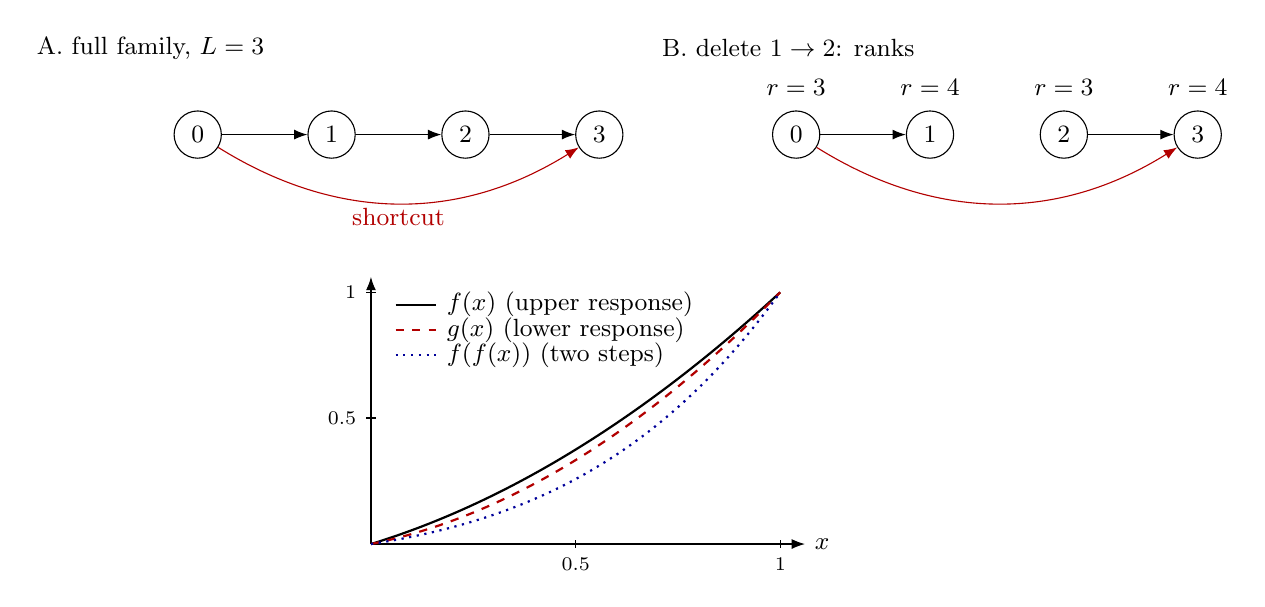
\begin{tikzpicture}[>=Latex,v/.style={circle,draw,minimum size=6mm,inner sep=0pt,font=\small}]
\begin{scope}
\node at (-0.6,1.1) {\small A.\ full family, $L=3$};
\node[v] (a0) at (0,0) {0};
\node[v] (a1) at (1.7,0) {1};
\node[v] (a2) at (3.4,0) {2};
\node[v] (a3) at (5.1,0) {3};
\draw[->] (a0)--(a1); \draw[->] (a1)--(a2); \draw[->] (a2)--(a3);
\draw[->,red!70!black] (a0) to[bend right=32] (a3);
\node[red!70!black,font=\small] at (2.55,-1.05) {shortcut};
\end{scope}
\begin{scope}[xshift=7.6cm]
\node at (-0.1,1.1) {\small B.\ delete $1\to2$: ranks};
\node[v] (b0) at (0,0) {0};
\node[v] (b1) at (1.7,0) {1};
\node[v] (b2) at (3.4,0) {2};
\node[v] (b3) at (5.1,0) {3};
\draw[->] (b0)--(b1); \draw[->] (b2)--(b3);
\draw[->,red!70!black] (b0) to[bend right=32] (b3);
\node[font=\small] at (0,0.6) {$r=3$};
\node[font=\small] at (1.7,0.6) {$r=4$};
\node[font=\small] at (3.4,0.6) {$r=3$};
\node[font=\small] at (5.1,0.6) {$r=4$};
\end{scope}
\begin{scope}[yshift=-5.2cm,xshift=2.2cm,x=5.2cm,y=3.2cm]
\draw[->] (0,0)--(1.06,0) node[right,font=\small] {$x$};
\draw[->] (0,0)--(0,1.06);
\foreach \t in {0.5,1} {\draw (\t,0.015)--(\t,-0.015) node[below,font=\scriptsize] {\t};}
\foreach \t in {0.5,1} {\draw (0.012,\t)--(-0.012,\t) node[left,font=\scriptsize] {\t};}
\draw[domain=0:1,samples=60,smooth,thick] plot (\x,{(\x+\x*\x)/2});
\draw[domain=0:1,samples=60,smooth,thick,red!70!black,dashed] plot (\x,{(\x+2*\x*\x)/3});
\draw[domain=0:1,samples=60,smooth,thick,blue!60!black,dotted] plot (\x,{((\x+\x*\x)/2+((\x+\x*\x)/2)*((\x+\x*\x)/2))/2});
\draw[thick] (0.06,0.95)--(0.16,0.95) node[right,font=\small] {$f(x)$ (upper response)};
\draw[thick,red!70!black,dashed] (0.06,0.85)--(0.16,0.85) node[right,font=\small,black] {$g(x)$ (lower response)};
\draw[thick,blue!60!black,dotted] (0.06,0.75)--(0.16,0.75) node[right,font=\small,black] {$f(f(x))$ (two steps)};
\end{scope}
\end{tikzpicture}
\caption{The construction for $L=3$ (four cores on four species). A: the path with its shortcut. B: after deleting the core $1\to2$ the ranks $r(i)=L+i$ for $i\le1$ and $r(i)=i+1$ for $i>1$ increase by one along every retained edge, including the shortcut, so Lemma~\ref{lem:graded} with $H=2L$ supplies a common state. Below: on $0<x<1$ the two-step response $f(f(x))$ lies strictly below the lower response $g(x)$ that the shortcut requires; the curves illustrate the exact identity~\eqref{eq:identity} and are not a numerical certificate.}
\label{fig:shortcut}
\end{figure}

\begin{proof}[Proof of Theorem~\ref{thm:order}]
(i) is Lemma~\ref{lem:pairPAC}.

(ii) Let $z\in\Rpos^n$ make every core productive and write $x_i=z_i$. Lemmas~\ref{lem:interval} and~\ref{lem:composition} applied to $P(0,1)$ and $P(1,2)$ give $x_2<g(x_0)$. Every productive edge strictly decreases the activity (Lemma~\ref{lem:interval}), so $x_L\le x_2$. The shortcut requires $x_L>g(x_0)$, a contradiction. No activity box was used.

(iii) By Lemma~\ref{lem:down} it suffices to treat the $n$ single deletions. If the shortcut is deleted, choose $r(i)=i$. If the path edge $j\to j+1$ is deleted, choose $r(i)=L+i$ for $i\le j$ and $r(i)=i+1$ for $i>j$. In both cases every retained path edge raises the rank by one, and so does the shortcut, since $r(0)=L$ and $r(L)=L+1$ in the second case. All ranks are at most $2L$. Lemma~\ref{lem:graded} with $H=2L$ gives a common state in $[9/10,1]^n$ that makes every retained core productive with positive currents, which is $\Comp_\Omega$ of the deletion.

(iv) Put $\delta=1/(1000(L-1))$ and
\[
a_0=\frac{19}{20},\qquad a_i=\frac{941}{1000}-(i-1)\delta\quad(1\le i\le L),
\]
so that $a_1=941/1000$ and $a_L=47/50$, the sequence decreases strictly, and $a_i\in[47/50,19/20]$. For every selected edge $s\to t$ (path or shortcut) we have $a_s>a_t\ge47/50>(19/20)^2\ge a_s^2$, so both currents $a_s-a_t$ and $a_t-a_s^2$ are positive.

(v) Keep $y_{X_i}=a_i$ on singleton complexes. Assign to the doubled complex $2X_0$ the single value $T_0=467/500$, and to $2X_i$, $1\le i\le L$, the value $T_i=a_i-\tfrac74\delta$; the complex $2X_L$ occurs in no reaction, and the uniform formula gives it a valid value as well. Since $0<\delta\le1/1000$ and $47/50\le a_i\le19/20$, all $T_i\in[81/100,1]$. The linear currents on an edge $s\to t$ are $p=a_s-a_t$ and $q=a_t-T_s$. On $0\to1$, $(p,q)=(9/1000,7/1000)$; on the shortcut $0\to L$, $(p,q)=(1/100,3/500)$; both use the same $T_0$ and satisfy $2q>p>q>0$. On every other path edge $i\to i+1$, $(p,q)=(\delta,\tfrac34\delta)$, with residuals $2q-p=\delta/2$ and $p-q=\delta/4$. Thus one global assignment makes all $2n$ linear currents positive and all $n$ cores productive.
\end{proof}

\begin{corollary}[No bounded-order local test]\label{cor:local}
For every $k\ge1$ there is a selected family (Construction~\ref{con:shortcut} with $n=k+1$) in which every subfamily of at most $k$ cores is compatible in a fixed box, the full family passes direction feasibility and independent-complex feasibility with witnesses in that box, and the full family is incompatible on the whole positive orthant. Hence no procedure that decides compatibility from the compatibility of all subfamilies of size at most $k$, together with the two relaxations, is correct on the class of unit-factor gain-two pair assemblies.
\end{corollary}

The corollary is a statement about the insufficiency of local tests. It is not a computational hardness result: the conflict has the short certificate~\eqref{eq:identity}, and a shortcut across a productive path of length at least two is simply a forbidden pattern in this class.

\begin{remark}[Dimension and Helly's theorem]\label{rem:helly}
For finitely many convex sets in $\R^d$, a minimally empty intersection has at most $d+1$ members \citep{helly1923,eckhoff1993}. This bounds the order of minimal conflicts only when the feasible sets of the cores are convex in a common space of \emph{fixed} dimension. Neither condition holds here. The feasible set of a pair is $\{(x,y):g(x)<y<f(x)\}$; its upper boundary $f$ is strictly convex, so the region below it, and hence the set, is not convex, and the same holds after a coordinatewise logarithm, where both boundaries become log-sum-exp functions. More simply, the ambient dimension is the number $n$ of species, which grows with the order, so even the Helly bound $n+1$ would not be violated. The theorem therefore exhibits genuinely collective conflicts within a growing number of shared variables; it makes no dimension-independent claim.
\end{remark}

For comparison, the same two-reaction cores arranged around a cycle give minimal conflicts of every order at the \emph{direction} layer.

\begin{proposition}[Ring: a direction-layer conflict of order $n$]\label{prop:ring}
For $n\ge3$ let the species be $X_i$, $i\in\Z/n\Z$, and the selected cores the $n$ pairs $P(i,i+1)$. Each core is a PAC. The full family fails direction feasibility on the whole orthant, hence is incompatible, while every proper subfamily is compatible in $[9/10,1]^n$.
\end{proposition}
\begin{proof}
PAC status is Lemma~\ref{lem:pairPAC}. A positive current on $X_i\rev X_{i+1}$ means $x_i>x_{i+1}$; around the cycle this gives $x_0>x_0$. Deleting $P(j,j+1)$ leaves the directed path $j+1\to j+2\to\dots\to j$ of $n-1$ edges; ranking its vertices $0,1,\dots,n-1$ in order and applying Lemma~\ref{lem:graded} with $H=n-1$ gives a common state. (For $n=3$ the channels are distinct; the formal statement is for the indexed presentation and every $n\ge2$.)
\end{proof}

The ring fails at the first obstruction layer of \citep{tcic2026}, the path with a shortcut only at the third. Both have order $n$.

\section{Exact elimination for bounded triangle fans}\label{sec:fan}

We now turn to the triangles of the predecessor and prove that, for any number of them sharing one reaction and any closed positive boxes, compatibility reduces exactly to one shared variable.

\begin{definition}[Fan data]\label{def:fan}
A \emph{fan} over a nonempty finite index set $I$ consists of integer gains $m_i\ge2$, a shared factor $b_0>0$, private factors $x_i,y_i>0$, private boxes $[\ell_i,u_i]$ with $0<\ell_i\le u_i$, and shared boxes $[\ell_A,u_A]$, $[\ell_B,u_B]$ with positive lower ends. Its network has species $A,B,C_i$ and reactions
\[
r_0\colon A\rev B\ (b_0),\qquad r_{i1}\colon B\rev C_i\ (x_i),\qquad r_{i2}\colon C_i\rev m_iA\ (y_i)\qquad(i\in I),
\]
and its selected cores are the triangles $T_i=(\{A,B,C_i\},\{r_0,r_{i1},r_{i2}\})$. The activity domain $\Omega$ is the product of all boxes.
\end{definition}

Write $a,b,c_i$ for the activities, $t_i=a^{m_i}$, $j=b_0(a-b)$ for the shared current, and $p_i=x_i(b-c_i)$, $q_i=y_i(c_i-t_i)$ for the private currents. The production residuals of $T_i$ are $m_iq_i-j$ at $A$, $j-p_i$ at $B$ and $p_i-q_i$ at $C_i$, so productivity of $T_i$ is the chain
\begin{equation}\label{eq:chain}
m_iq_i>j>p_i>q_i .
\end{equation}

\begin{lemma}[Triangles are PACs; directions are automatic]\label{lem:trianglePAC}
Each $T_i$ is a PAC of the fan network. Moreover~\eqref{eq:chain} implies $q_i>0$, hence $j,p_i,q_i>0$: the direction clause of Definition~\ref{def:family} is implied by productivity.
\end{lemma}
\begin{proof}
Side incidence is immediate and $(j,p_i,q_i)=(1,5/6,2/3)$ is productive since $m_i\ge2$. Any strict submotif that is side-incident contains the endpoints of each of its reactions; a proper subset of the three reactions is a path in the cycle $A\to B\to C_i\to A$, and for any signed flow on a path some endpoint species has production of the wrong sign or two adjacent productions of opposite signs, so no proper reaction subset is productive, while the full reaction set forces all three species. If $q_i\le0$ then $m_iq_i\le q_i$ (as $m_i\ge1$), contradicting $m_iq_i>j>p_i>q_i$.
\end{proof}

\begin{lemma}[Private elimination]\label{lem:private}
Fix $a,b$ and $i\in I$, and write $x=x_i$, $y=y_i$, $m=m_i$, $t=a^{m}$, $\ell=\ell_i$, $u=u_i$. There is $c\in[\ell,u]$ with~\eqref{eq:chain} if and only if the following five strict comparisons hold:
\begin{equation}\label{eq:five}
xy(b-t)<(x+y)j<mxy(b-t),\qquad (x+y)\ell<xb+yt,\qquad xb-j<xu,\qquad myt+j<myu .
\end{equation}
\end{lemma}
\begin{proof}
Solving~\eqref{eq:chain} for $c$ gives the open interval
\[
\max\Bigl(b-\frac{j}{x},\ t+\frac{j}{my}\Bigr)<c<\frac{xb+yt}{x+y}.
\]
An open interval $(\lambda,\upsilon)$ meets a nonempty closed interval $[\ell,u]$ exactly when $\lambda<\upsilon$, $\ell<\upsilon$ and $\lambda<u$: necessity is clear, and for sufficiency clamp $(\lambda+\upsilon)/2$ to $[\ell,u]$ and note that the three comparisons keep the clamped point strictly between $\lambda$ and $\upsilon$; the case $\ell=u$ is included. Applying this with $\lambda$ the maximum of the two lower bounds and clearing the positive denominators gives~\eqref{eq:five}.
\end{proof}

Substituting $j=b_0(a-b)$ into~\eqref{eq:five} and solving each comparison for $b$ yields, at fixed $a$, three lower and two upper \emph{responses} with positive constant denominators:
\begin{align}
L_{i1}(a)&=\frac{(x_i+y_i)b_0a+m_ix_iy_it_i}{m_ix_iy_i+(x_i+y_i)b_0}, &
L_{i2}(a)&=\frac{(x_i+y_i)\ell_i-y_it_i}{x_i}, &
L_{i3}(a)&=\frac{b_0a+m_iy_i(t_i-u_i)}{b_0},\label{eq:lower}\\
U_{i1}(a)&=\frac{(x_i+y_i)b_0a+x_iy_it_i}{x_iy_i+(x_i+y_i)b_0}, &
U_{i2}(a)&=\frac{x_iu_i+b_0a}{x_i+b_0}. \label{eq:upper}
\end{align}

\begin{theorem}[Bounded fan elimination]\label{thm:fan}
For a fan over a nonempty $I$ with $\ell_B\le u_B$, the full family is compatible if and only if there is $a\in[\ell_A,u_A]$ such that
\begin{equation}\label{eq:univariate}
L_{ir}(a)<U_{ks}(a),\qquad \ell_B<U_{ks}(a),\qquad L_{ir}(a)<u_B
\end{equation}
for all $i,k\in I$, $r\in\{1,2,3\}$ and $s\in\{1,2\}$. When these hold, a common $b$ and then every $c_i$ are reconstructed by the clamping rule of Lemma~\ref{lem:private}, and the resulting vector lies in $\Omega$ and satisfies Definition~\ref{def:family} for the whole fan.
\end{theorem}
\begin{proof}
By Lemma~\ref{lem:private}, at fixed $(a,b)$ the whole fan is feasible with private activities in their boxes if and only if all $5|I|$ comparisons~\eqref{eq:five} hold, that is, $\max_{i,r}L_{ir}(a)<b<\min_{k,s}U_{ks}(a)$. The interval fact of Lemma~\ref{lem:private} with $[\ell,u]=[\ell_B,u_B]$ turns the existence of such a $b$ in the shared box into~\eqref{eq:univariate}, and produces one common $b$ when they hold. Applying the interval fact once more to each private interval reconstructs every $c_i$. Positivity of all coordinates comes from the boxes, and the direction clause from Lemma~\ref{lem:trianglePAC}.
\end{proof}

For rational data the comparisons~\eqref{eq:univariate} are strict polynomial inequalities in $a$ of degree at most $\max_i m_i$ after clearing positive constants, so exact real-algebraic decision methods apply. The formal theorem certifies the reduction and the reconstruction; it does not certify any particular root-isolation implementation.

\section{A robust three-core fan}\label{sec:robust}

Theorem~\ref{thm:fan} makes it possible to search for minimal conflicts among fans by looking at crossings of the eliminated response curves. The following instance was found that way and then proved exactly. Take $b_0=1$, shared boxes $A,B\in[1/10,9/10]$, and private data
\begin{center}
\begin{tabular}{@{}lcccl@{}}
\toprule
branch $i$ & gain $m_i$ & factor $x_i$ & factor $y_i$ & private box $[\ell_i,u_i]$ \\
\midrule
0 & 3 & 4 & 2 & $[13/20,\ 71/100]$ \\
1 & 4 & 1/2 & 1 & $[13/20,\ 19/25]$ \\
2 & 3 & 1 & 1 & $[13/20,\ 19/25]$ \\
\bottomrule
\end{tabular}
\end{center}

\begin{theorem}[Simultaneous robustness]\label{thm:robust}
This fan is minimally incompatible. It remains minimally incompatible when all seven factors $b_0,x_i,y_i$ and all ten box endpoints are varied independently by absolute amounts at most $\rho=10^{-6}$, keeping the gains fixed and one common shared factor. Throughout this cube the full family passes direction feasibility with an interior witness and independent-complex feasibility with one global assignment satisfying the induced individual complex bounds. In particular the phenomenon holds on an open set of parameters.
\end{theorem}

The proof rests on a uniform negative margin at the reference factors.

\begin{lemma}[Uniform negative margin]\label{lem:margin}
At the reference factors, let $\tau$ be the minimum of the nine production residuals at a state with $A\ge0$, $C_0\le89/125$ and $C_1\ge81/125$. Then $\tau\le-3/500$.
\end{lemma}
\begin{proof}
Write $u=C_0$ and $\ell=C_1$. Three residual identities are
\[
P_{0B}=A-5B+4C_0,\qquad P_{1C}=\frac B2-\frac{3C_1}{2}+A^4,\qquad 2P_{2A}+3P_{2C}=5B-2A-3A^3 ,
\]
where $P_{iS}$ is the residual of branch $i$ at species $S$. Since every residual is at least $\tau$ (even when $\tau<0$),
\[
5B\le A+4u-\tau,\qquad B+2A^4\ge3\ell+2\tau,\qquad 5B-2A-3A^3\ge5\tau .
\]
Put $a_*=7/8$. If $0\le A\le a_*$, combine the first two inequalities and monotonicity of $A^4$; if $A\ge a_*$, combine the first and third and monotonicity of $A^3$. Respectively,
\[
11\tau\le a_*+4u+10a_*^4-15\ell,\qquad 6\tau\le4u-a_*-3a_*^3 .
\]
At the worst allowed endpoints $u=89/125$, $\ell=81/125$ the right-hand sides divided by $11$ and $6$ equal $-34607/2816000$ and $-2353/384000$, both below $-3/500$.
\end{proof}

At the reference boxes ($u\le71/100$, $\ell\ge13/20$) the three necessary inequalities $5B<71/25+A$, $39/20<B+2A^4$ and $2A+3A^3<5B$ have no solution with $A\ge0$; the split at $A=7/8$ gives the exact gaps $8867/256000$ and $573/12800$. This is a universal algebraic contradiction, not an optimizer's estimate.

\begin{figure}[t]
\centering
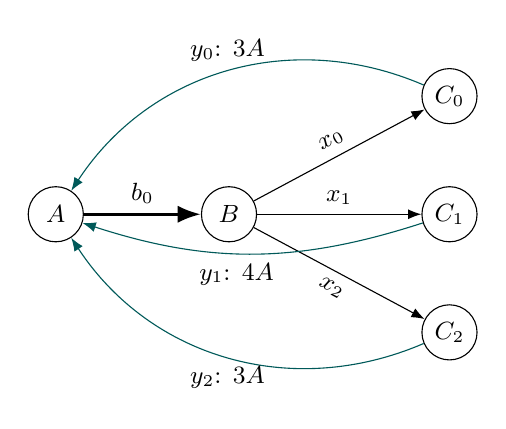
\begin{tikzpicture}[>=Latex,v/.style={circle,draw,minimum size=7mm,inner sep=0pt,font=\small}]
\node[v] (A) at (0,0) {$A$};
\node[v] (B) at (2.2,0) {$B$};
\node[v] (C0) at (5.0,1.5) {$C_0$};
\node[v] (C1) at (5.0,0) {$C_1$};
\node[v] (C2) at (5.0,-1.5) {$C_2$};
\draw[->,very thick] (A)--(B) node[midway,above,font=\small] {$b_0$};
\draw[->] (B)--(C0) node[midway,above,sloped,font=\small] {$x_0$};
\draw[->] (B)--(C1) node[midway,above,font=\small] {$x_1$};
\draw[->] (B)--(C2) node[midway,below,sloped,font=\small] {$x_2$};
\draw[->,teal!70!black] (C0) to[bend right=40] node[midway,above,font=\small,black] {$y_0$: $3A$} (A);
\draw[->,teal!70!black] (C1) to[bend left=18] node[pos=0.55,below,font=\small,black] {$y_1$: $4A$} (A);
\draw[->,teal!70!black] (C2) to[bend left=40] node[midway,below,font=\small,black] {$y_2$: $3A$} (A);
\end{tikzpicture}
\caption{The robust fan. One shared reaction $A\rev B$ carries the same current $j=b_0(a-b)$ in all three triangles; each branch returns to $m_iA$ through its private species. Deleting any one branch leaves a compatible pair; all three together force the contradictory bounds of Lemma~\ref{lem:margin}.}
\label{fig:fan}
\end{figure}

\begin{proof}[Proof of Theorem~\ref{thm:robust}]
\emph{Deletion witnesses.} With $\eta=10^{-5}$ and an omitted private coordinate set to $7/10$, the states
\begin{center}
\begin{tabular}{@{}lccl@{}}
\toprule
retained pair & $A$ & $B$ & active private activities \\
\midrule
$\{0,1\}$ & $141/160$ & $93/125$ & $C_0=71/100-\eta$, $C_1=13/20+\eta$ \\
$\{0,2\}$ & $169/200$ & $88/125$ & $C_0=67/100$, $C_2=653/1000$ \\
$\{1,2\}$ & $22/25$ & $157/200$ & $C_1=13/20+\eta$, $C_2=18/25$ \\
\bottomrule
\end{tabular}
\end{center}
have, in the table's order, minimum retained residuals $311253/3276800000$, $10809/8000000$ and $429509/25000000$, all exceeding $9/100000$, and every coordinate lies at least $\eta$ inside both endpoints of its original box.

\emph{Perturbation control.} Perturbed boxes remain nonempty and inside $(0,1)$, and perturbed factors remain positive. At a state in these boxes every monomial lies in $[0,1]$, so if a factor changes by at most $\rho$ its current changes by at most $\rho$, the difference of its two complex activities having absolute value at most one. Each residual is $mq-j$, $j-p$ or $p-q$ with $m\le4$, so its total absolute current coefficient is at most five and its change is at most $5\rho$.

\emph{Incompatibility in the cube.} Suppose the perturbed full family were compatible at some state. The perturbed upper endpoint of $C_0$ is at most $71/100+\rho\le89/125$ and the perturbed lower endpoint of $C_1$ is at least $13/20-\rho\ge81/125$, so Lemma~\ref{lem:margin} applies to the reference-factor residuals at that state: some reference residual is at most $-3/500$, hence the corresponding perturbed residual is at most $-3/500+5\rho<0$, contradicting productivity.

\emph{Deletions in the cube.} Each listed witness remains inside every perturbed box because $\eta>\rho$, and its retained residuals exceed $9/100000-5\rho>0$. By Lemma~\ref{lem:down} every proper subfamily is compatible.

\emph{Directions.} $A=17/20$, $B=3/4$, $C_i=7/10$ are interior and satisfy $A>B>C_i>A^{m_i}$; positive factor changes preserve the signs.

\emph{Independent complexes.} Take
\[
A=\frac{9}{10}-\eta,\qquad B=\frac{37}{50},\qquad (C_0,C_1,C_2)=\Bigl(\frac{701}{1000},\frac{651}{1000},\frac{341}{500}\Bigr),\qquad T_3=\frac{157}{250},\qquad T_4=\frac{61}{100},
\]
where $T_3$ is the shared value of the complex $3A$ (used by branches 0 and 2) and $T_4$ that of $4A$. The minimum reference residual is $201/100000$, and the same $5\rho$ estimate keeps all residuals positive in the cube; positivity of all currents then follows from Lemma~\ref{lem:trianglePAC}. The induced individual bounds survive: $(1/10+\rho)^m<T_m<(9/10-\rho)^m$ for $m=3,4$ by direct rational comparison.
\end{proof}

The obstruction is a monomial-layer one in the sense of \citep{tcic2026}: the missing equations are exactly $T_3=A^3$ and $T_4=A^4$, and Lemma~\ref{lem:margin} uses only the monotonicity of these two monomials on $A\ge0$ across the separator $A=7/8$.

\begin{proposition}[A two-parameter forbidden window]\label{prop:window}
Keep the kinetics and gains above and the shared boxes $[1/10,9/10]$. Replace the upper endpoint of branch 0's box by $u$ and the lower endpoint of branch 1's box by $\ell$. For every $71/100\le u\le89/125$ and $81/125\le\ell\le13/20$ the family is minimally incompatible.
\end{proposition}
\begin{proof}
The full family would give $5B<356/125+A$, $243/125<B+2A^4$ and $2A+3A^3<5B$, contradicted by the same split at $A=7/8$ (Lemma~\ref{lem:margin} with $\tau=0$). The private boxes only expand, so the deletion witnesses of the reference family, with omitted coordinates at their original lower bounds ($C_0=71/100$, $C_1=13/20$ on the box faces are allowed), remain valid.
\end{proof}

Table~\ref{tab:relax} summarizes which requirements each description retains and what certifies its verdict, for the two headline families.

\begin{table}[t]
\centering
\small
\begin{tabular}{@{}>{\raggedright\arraybackslash}p{0.23\linewidth}>{\raggedright\arraybackslash}p{0.30\linewidth}>{\raggedright\arraybackslash}p{0.41\linewidth}@{}}
\toprule
Description & Constraints retained or removed & Verdict and certificate \\
\midrule
Full family, physical & all production and direction requirements; $y_c=z^c$ & \textbf{infeasible}: identity~\eqref{eq:identity} (path); margin $\tau\le-3/500$ (fan) \\
Proper subfamily & one core's requirements removed; boxes, factors, shared currents unchanged & \textbf{feasible}: graded state~\eqref{eq:state} (path); explicit rational pair states (fan) \\
Direction feasibility $\DIR_\Omega$ & only current signs, at a physical state in the box & \textbf{feasible}: $a_i$ decreasing with $a_i>a_s^2$ (path); $A>B>C_i>A^{m_i}$ (fan) \\
Independent-complex feasibility $\LIN$ & currents and productions linear in complex values; coupling $y_c=z^c$ removed & \textbf{feasible}: single global assignment with $T_0=467/500$ shared by both edges from $X_0$ (path); shared $T_3$ (fan) \\
\bottomrule
\end{tabular}
\caption{What each relaxation forgets. Both relaxations pass at the full family, so the conflict lives entirely in the monomial coupling between complexes of the same species.}
\label{tab:relax}
\end{table}

\section{Graded assemblies and constructive recognition}\label{sec:graded}

Lemma~\ref{lem:graded} does not depend on the path structure of Section~\ref{sec:order}. A \emph{pair assembly} is a finite directed multigraph $G=(V,E,\mathrm{src},\mathrm{dst})$ with $\mathrm{src}(e)\ne\mathrm{dst}(e)$, each edge $e$ carrying the literal two-reaction core $P(\mathrm{src}(e),\mathrm{dst}(e))$ with unit factors; its network has $2|E|$ reactions on the species $V$, and a species may occur in many cores.

\begin{theorem}[Graded gluing]\label{thm:graded}
Let $G$ be a pair assembly and suppose there are integer ranks $r\colon V\to\{0,\dots,H\}$ with $r(\mathrm{dst}(e))=r(\mathrm{src}(e))+1$ for every edge. Then every edge core is a PAC, and the state~\eqref{eq:state} lies in $[9/10,1]^V$, makes every edge core productive and makes all $2|E|$ currents positive. In particular the full family is compatible in $[9/10,1]^V$.
\end{theorem}
\begin{proof}
Lemmas~\ref{lem:pairPAC} and~\ref{lem:graded}; each shared species receives the single value $x_v$.
\end{proof}

\begin{figure}[t]
\centering
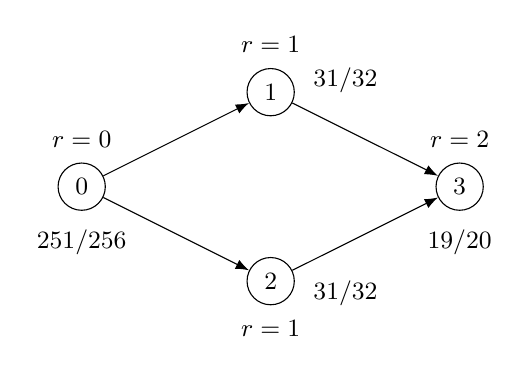
\begin{tikzpicture}[>=Latex,v/.style={circle,draw,minimum size=6mm,inner sep=0pt,font=\small}]
\node[v] (n0) at (0,0) {0};
\node[v] (n1) at (2.4,1.2) {1};
\node[v] (n2) at (2.4,-1.2) {2};
\node[v] (n3) at (4.8,0) {3};
\draw[->] (n0)--(n1); \draw[->] (n0)--(n2); \draw[->] (n1)--(n3); \draw[->] (n2)--(n3);
\node[font=\small] at (0,0.6) {$r=0$};
\node[font=\small] at (2.4,1.8) {$r=1$};
\node[font=\small] at (2.4,-1.8) {$r=1$};
\node[font=\small] at (4.8,0.6) {$r=2$};
\node[font=\small] at (0,-0.7) {$251/256$};
\node[font=\small] at (3.35,1.35) {$31/32$};
\node[font=\small] at (3.35,-1.35) {$31/32$};
\node[font=\small] at (4.8,-0.7) {$19/20$};
\end{tikzpicture}
\caption{A graded diamond, $H=2$. Each arrow is a two-reaction core, not a single reaction. The rational states $251/256$, $31/32$, $31/32$, $19/20$ from~\eqref{eq:state} make all four cores productive simultaneously; species $0$ and $3$ each belong to two cores and receive one value.}
\label{fig:graded}
\end{figure}

\begin{theorem}[Constructive recognition]\label{thm:recognition}
Given an explicitly listed finite directed graph, one can decide in polynomial time whether it admits integer ranks increasing by one along every edge and, if so, output such ranks and a common rational productive state of polynomial bit length. A rejection asserts only that the graph is not graded.
\end{theorem}
\begin{proof}
Traverse each connected component of the underlying undirected graph from an initial vertex of rank $0$, propagating $+1$ along an edge traversed in its direction and $-1$ against it, and check every previously ranked vertex for consistency. Any mismatch violates the necessary rank equation on some edge; if none occurs all edges satisfy it. Subtract the minimum rank in each component. The rank difference of two vertices in a component of $v$ vertices is the signed sum along a simple undirected path, so normalized ranks lie in $\{0,\dots,H\}$ with $H\le|V|-1$. Apply Lemma~\ref{lem:graded}: a coordinate with exponent $d$ equals $(20\cdot8^d-5^d)/(20\cdot8^d)$, of $O(|V|)$ bits, computable by integer arithmetic. The traversal takes $O(|V|+|E|)$ graph operations on $O(\log|V|)$-bit ranks.
\end{proof}

Grading is a sufficient structural class with an exact constructive certificate; the theorem makes no claim that nongraded assemblies are incompatible. Acyclicity alone does not suffice: the path with a shortcut is acyclic and incompatible. In the box $[9/10,1]$ the failure is quantitative: for a productive edge with $x=1-\varepsilon$, $y=1-\varepsilon'$, the response interval gives $1-f(x)=\varepsilon(3-\varepsilon)/2$ and $1-g(x)=\varepsilon(5-2\varepsilon)/3$, so $\frac{29}{20}\varepsilon<\varepsilon'<\frac53\varepsilon$; two successive edges multiply $\varepsilon$ by more than $(29/20)^2=2.1025$ while their shortcut requires a factor below $5/3$, and $(29/20)^2-5/3=523/1200>0$.

\section{Chemical interpretation and scope}\label{sec:chemistry}

\paragraph{Food adapter.} The pair~\eqref{eq:pair} is written in effective internal-species form. It admits the mass-balanced open-system reading $X_s\rev X_t$, $X_t+F\rev 2X_s$ with a food species $F$ held at activity one: assigning unit mass to every internal species and to $F$ balances both channels, and unit standard-state factors give exactly the currents $p=x_s-x_t$ and $q=x_t\cdot1-x_s^2$ used above. In the independent-complex relaxation the value of the complex $X_t+F$ is the value assigned to $X_t$. Likewise a triangle $A\rev B\rev C\rev mA$ reads as $C+(m-1)F\rev mA$. This is an interpretation of the effective equations, not a change to the formal predicates, and it does not claim that a closed system produces all species indefinitely.

\paragraph{Mechanism.} The conflict of Theorem~\ref{thm:order} is one of nonlinear consistency: the complex $2X_s$ must have activity $x_s^2$, so a productive step from $x$ lands in $(g(x),f(x))$ and two steps land below $g(x)$. Independent complex variables erase precisely the equation $y_{2X_s}=x_s^2$, and the witness of part~(v) exploits that erasure while keeping one value per complex. Sparse local structure, a fixed species box for all proper-subfamily witnesses, and globally feasible linear tests do not repair the missing constraint. The fan of Section~\ref{sec:robust} conflicts in the same layer through the monotonicity of $A^3$ and $A^4$.

\paragraph{What is not claimed.} These are static compatibility results. They do not establish persistence, boundary repulsion, long-time simultaneous activity, stochastic establishment, extinction or switching rates. Theorem~\ref{thm:robust} concerns a neighbourhood in the space of kinetic factors and box endpoints, not robustness of an attractor. No complexity lower bound follows from the large minimal conflicts, which have short exact certificates. No frequency of such conflicts in random networks is asserted, since no probability model is specified. A classification of all finite networks is outside the claims proved here.

\section{Formal verification}\label{sec:formal}

All statements marked as formal in Table~\ref{tab:lean} have been compiled in Lean~4 \citep{demoura2021}, toolchain \lean{leanprover/lean4:v4.30.0}, against Mathlib \citep{mathlib2020} with a frozen \lean{lake-manifest} (Table~\ref{tab:receipts}). Verification treats every warning as an error, rejects \lean{sorry}, extracts the requested declaration signatures, reports the axioms used, and records SHA-256 hashes of the source files. Every verified declaration depends only on the standard axioms \lean{propext}, \lean{Classical.choice} and \lean{Quot.sound}.

\subsection{Architecture}

The development extends the namespace \lean{ThermoCoreCompatibility} of \citep{tcic2026}, whose \lean{Reaction.lean}, \lean{Source.lean}, \lean{CoreFamily.lean}, \lean{Direction.lean} and \lean{Toric.lean} supply Definitions~\ref{def:crn}--\ref{def:motif} and the two relaxation predicates. The new material, about $1{,}900$ lines in $23$ files under \lean{Hypergraph/}, is organized as follows.
\begin{itemize}[before=\sloppy]
\item \lean{PrivateTriangleBounds.lean}, \lean{TriangleSource.lean}: Lemma~\ref{lem:private} (\lean{privateTriangle_box_iff}, \lean{privateTriangle_box_iff_polynomial}), the literal triangle structure \lean{TriangleIn}, its production characterization and signed PAC minimality (\lean{TriangleIn.isPAC}, Lemma~\ref{lem:trianglePAC}).
\item \lean{FanElimination.lean}, \lean{FiniteBounds.lean}, \lean{FanUnivariate.lean}, \lean{FanSource.lean}, \lean{FanSourceTheorem.lean}: the fan data type \lean{FanData}, the responses~\eqref{eq:lower}--\eqref{eq:upper} (\lean{FanData.lowerBound}, \lean{FanData.upperBound}), the univariate conditions~\eqref{eq:univariate} and Theorem~\ref{thm:fan} at the source level (\lean{FanData.sourceCompatible_univariate_iff}).
\item \lean{RingHyperedge.lean}, \lean{RingSource.lean}: the pair productivity predicate \lean{Ring.Productive}, the local deletion step, and Proposition~\ref{prop:ring} on $\Z/n$ for every $n\ge2$ (\lean{Ring.source_isPAC}, \lean{Ring.source_full_incompatible}, \lean{Ring.source_deletion}).
\item \lean{GradedGluing.lean}, \lean{GradedSource.lean}: Lemma~\ref{lem:graded} (\lean{Graded.state}, \lean{Graded.edge_productive}, \lean{Graded.graded_common_state}), the pair assembly \lean{PairAssembly} with its PAC proof, Theorem~\ref{thm:graded} (\lean{PairAssembly.graded_source_compatible}) and the boxed shortcut obstruction (\lean{Graded.shortcut_obstruction}).
\item \lean{PairResponseBounds.lean}, \lean{ShortcutPathSource.lean}, \lean{ShortcutPathRelaxations.lean}, \lean{UnboundedMonomialOrder.lean}: Lemmas~\ref{lem:interval} and~\ref{lem:composition} (\lean{PairResponse.interval_iff}, \lean{composition_identity}, \lean{composition_lt}, \lean{path_incompatible}), Construction~\ref{con:shortcut} (\lean{Shortcut.assembly}), the deletion ranks (\lean{Shortcut.rank_edge}), and Theorem~\ref{thm:order} (\lean{Shortcut.unbounded_monomial_order}).
\item \lean{MonomialTriple.lean}, \lean{MonomialTripleSource.lean}, \lean{MonomialTripleWindow.lean}, \lean{TripleMargin.lean}, \lean{TriplePerturbation.lean}, \lean{TripleRobustSource.lean}: the reference fan \lean{MonomialTriple.data}, its incompatibility and deletions, its \lean{DirectionCompatible} and \lean{LinearComplexCompatible} witnesses, Proposition~\ref{prop:window} (\lean{minimal_triple_parameter_region}), Lemma~\ref{lem:margin} (\lean{negative_margin}, \lean{source_coordinate_margin}), the current and residual perturbation bounds, and Theorem~\ref{thm:robust} (\lean{simultaneous_perturbation}).
\item \lean{Main.lean} packages the original campaign root \lean{tcch_resolution}; \lean{Reviewed.lean} packages it with the two arbitrary-order and robustness theorems as \lean{reviewed_resolution}.
\end{itemize}

The two new fields of the strict root are stated for every $L\ge2$ and every fan in the perturbation cube:
\begin{lstlisting}
structure ReviewedResolution : Prop where
  original : TCCHResolution
  unbounded_order : ∀ (L : ℕ) (hL : 2 ≤ L),
    (∀ e, ((Shortcut.assembly L hL).motif e).IsPAC) ∧
    (¬ ∃ z : Fin (L+1) → ℝ, (∀ i, 0 < z i) ∧
      ∀ e, ((Shortcut.assembly L hL).motif e).Productive
        ((Shortcut.assembly L hL).network.current z)) ∧
    (∀ F, F ≠ Set.univ → Shortcut.Compatible L hL F) ∧
    (∃ z : Fin (L+1) → ℝ, (∀ i, 9/10 ≤ z i ∧ z i ≤ 1) ∧
      ∀ r, 0 < (Shortcut.assembly L hL).network.current z r) ∧
    (Shortcut.family L hL).LinearComplexCompatible ∧
    (∀ i, 9/10 ≤ Shortcut.complexValues L (atom i 1) ∧
      Shortcut.complexValues L (atom i 1) ≤ 1) ∧
    (∀ i, 81/100 ≤ Shortcut.complexValues L (atom i 2) ∧
      Shortcut.complexValues L (atom i 2) ≤ 1)
  robust_triple : ∀ (D : FanData (Fin 3)) (la ua lb ub : ℝ),
    MonomialTriple.Near D la ua lb ub →
      (¬ D.SourceCompatible Set.univ la ua lb ub) ∧
      ∀ j : Fin 3, D.SourceCompatible {i | i ≠ j} la ua lb ub

theorem reviewed_resolution : ReviewedResolution :=
  ⟨tcch_resolution, Shortcut.unbounded_monomial_order,
   MonomialTriple.simultaneous_perturbation⟩
\end{lstlisting}
Here \lean{Shortcut.Compatible L hL F} is $\Comp_{[9/10,1]^n}(F)$ stated with productivity only, which for pairs implies the direction clause (Lemma~\ref{lem:interval}); \lean{FanData.SourceCompatible} includes both clauses and all boxes explicitly; and \lean{MonomialTriple.Near D la ua lb ub} says that the gains agree with the reference data and that each of the seven factors and ten endpoints is within $10^{-6}$ of its reference value. The original root \lean{TCCHResolution} contains Theorem~\ref{thm:fan}, Proposition~\ref{prop:ring}, the reference fan with both relaxation witnesses, Proposition~\ref{prop:window}, and Theorem~\ref{thm:graded}.

\subsection{Concordance}

\begin{table}[t]
\centering
\small
\begin{tabular}{@{}>{\raggedright\arraybackslash}p{0.27\linewidth}>{\raggedright\arraybackslash}p{0.69\linewidth}@{}}
\toprule
Statement & Lean declaration (namespace \lean{ThermoCoreCompatibility.Hypergraph}) \\
\midrule
Lemma~\ref{lem:pairPAC} & \lean{PairAssembly.source_isPAC}, \lean{Ring.source_isPAC} \\
Lemma~\ref{lem:interval} & \lean{PairResponse.interval_iff}, \lean{PairResponse.domain} \\
Lemma~\ref{lem:composition} & \lean{PairResponse.composition_identity}, \lean{composition_lt}, \lean{f_mono}, \lean{two_step} \\
Lemma~\ref{lem:graded} & \lean{Graded.state_bounds}, \lean{Graded.edge_productive}, \lean{Graded.graded_common_state} \\
Theorem~\ref{thm:order} (i)--(v) & \lean{Shortcut.unbounded_monomial_order}; ingredients \lean{Shortcut.assembly}, \lean{rank_edge}, \lean{source_deletion}, \lean{source_full_incompatible} (via \lean{PairResponse.path_incompatible}), \lean{scalar_relaxations}, \lean{source_directions}, \lean{source_relaxed} \\
Example~\ref{ex:three} & instance $L=2$ of the above; the printed rationals are checked by \lean{check_paper.py} \\
Corollary~\ref{cor:local} & conventional deduction from Theorem~\ref{thm:order} \\
Proposition~\ref{prop:ring} & \lean{Ring.source_full_incompatible}, \lean{Ring.source_deletion} (all $n\ge2$, indexed presentation) \\
Lemma~\ref{lem:trianglePAC} & \lean{TriangleIn.isPAC}, \lean{triangle_currents_positive} \\
Lemma~\ref{lem:private} & \lean{private_interval_box_iff}, \lean{privateTriangle_box_iff}, \lean{privateTriangle_box_iff_polynomial} \\
Theorem~\ref{thm:fan} & \lean{FanData.privateConditions_iff_bounds}, \lean{FanData.commonB_iff}, \lean{FanData.sourceCompatible_univariate_iff} \\
Lemma~\ref{lem:margin} & \lean{MonomialTriple.negative_margin}, \lean{source_coordinate_margin} (formal $\tau$ is any common lower bound) \\
Theorem~\ref{thm:robust}, incompatibility and deletions in the cube & \lean{MonomialTriple.simultaneous_perturbation}; \lean{current_perturbation}, \lean{production_perturbation}, \lean{residual_error}, \lean{stable_source_witness} \\
Theorem~\ref{thm:robust}, relaxations at the reference data & \lean{MonomialTriple.source_directionCompatible}, \lean{source_linearComplexCompatible} \\
Proposition~\ref{prop:window} & \lean{MonomialTriple.minimal_triple_parameter_region} \\
Theorem~\ref{thm:graded} & \lean{PairAssembly.graded_source_compatible}; boxed shortcut obstruction \lean{Graded.shortcut_obstruction} \\
Theorem~\ref{thm:recognition} & conventional; exact implementation \lean{graded()} in \lean{check_paper.py} \\
\bottomrule
\end{tabular}
\caption{Correspondence between the statements of this paper and the formal declarations.}
\label{tab:lean}
\end{table}

Table~\ref{tab:lean} lists the principal declaration behind each statement. Two semantic details deserve mention. The formal total complex function \lean{Shortcut.complexValues} assigns a value to \emph{every} complex, not only to an edge-indexed list; the unused doubled complex $2X_L$ receives the uniform-formula value $a_L-\tfrac74\delta$, which enters no current and satisfies the same bound. And the formal relaxation witness of the reference fan uses $A=9/10$ exactly, whereas the proof of Theorem~\ref{thm:robust} uses $A=9/10-\eta$ so that the witness stays interior under box perturbation.

\subsection{Receipts}

The strict root \lean{reviewed_resolution} was verified with exit code $0$, empty compiler output, and the three standard axioms; the original root \lean{tcch_resolution} was re-verified unchanged. Table~\ref{tab:receipts} lists the SHA-256 values of the two root source files, of the two new source modules behind Theorems~\ref{thm:order} and~\ref{thm:robust}, of the frozen manifest, and of the two receipt files that bind the toolchain, manifest and per-module source hashes; the full per-file hash list is recorded in the evidence manifest accompanying the sources. A public release tag and archive DOI of the Lean sources remain a pre-submission step.

\begin{table}[t]
\centering
\begin{tabular}{@{}ll@{}}
\toprule
File & SHA-256 \\
\midrule
\lean{Reviewed.lean} (strict root) & \hash{61d86208044db05c46a0e65b2685aec594d6f536e1bbf5401e9ef0db72f9977d} \\
\lean{Main.lean} (original root) & \hash{ec9715043ff52a9687217dcbedc6b5d3ee0aa15d311355595d8d8e608b963661} \\
\lean{UnboundedMonomialOrder.lean} & \hash{244e11c5a7395f2081d62e0d3d134aef770b45dc90d628db742f63e0e6040cc5} \\
\lean{TripleRobustSource.lean} & \hash{58ca717cb198b855d5952d15a5dd12407eef14028153d679c831ee76153585ad} \\
\lean{lake-manifest.json} & \hash{a8df0b606ec258561c226df89856884be433c19b49fb0a27335d69bb2b6e9fac} \\
\lean{reviewed_receipt.json} & \hash{64b3baf15cf15946fe10d48a032039a809d027921fba9f18f79287702c068f5b} \\
\lean{root_receipt.json} & \hash{f557fd3fc12c7c4f1ae1cf5919bd061bb287cb4122cdd771dde6777cef5f7633} \\
\bottomrule
\end{tabular}
\caption{SHA-256 receipts of the strict verification runs (toolchain \texttt{leanprover/lean4:v4.30.0}).}
\label{tab:receipts}
\end{table}

\subsection{What is proved by hand}\label{sec:notformal}

The following statements are proved in this paper but are not part of the formal development.
\begin{enumerate}
\item Channel distinctness for $n\ge3$, the counting of species--core incidences, and acyclicity in Construction~\ref{con:shortcut}; the formal statements use finite indexed types.
\item Corollary~\ref{cor:local} and Remark~\ref{rem:helly}.
\item In Theorem~\ref{thm:robust}, the persistence of the direction and independent-complex witnesses throughout the perturbation cube, including the induced complex bounds; these are conventional consequences of the same $5\rho$ estimate, checked at the reference values by exact arithmetic. The compiled theorem \lean{simultaneous_perturbation} states incompatibility and all deletions in the cube; the relaxation witnesses are compiled at the reference data only.
\item Positivity and nonemptiness of all perturbed factors and boxes, which are immediate inequalities.
\item Theorem~\ref{thm:recognition}: the traversal algorithm and its complexity bound; the exact implementation in \lean{check_paper.py} is tested on controls, not verified.
\item The food adapter and the physical reading of Section~\ref{sec:chemistry}.
\end{enumerate}
The script \lean{check_paper.py}, distributed with the sources, replays in exact rational arithmetic every number printed in this paper, including $42$ path deletion states for $L\in\{2,3,4,8,20\}$, the fan witnesses and margins, and the graded diamond; it guards transcription and proves nothing universal.

\section{Discussion}\label{sec:discussion}

\paragraph{Local tests and layers.} The main lesson is that thermodynamic compatibility of interacting cores is not a bounded-order property. With direction feasibility alone, the ring shows conflicts of every order; with both global relaxations adjoined, the path with a shortcut still does. In every case the certificate is short, so the results say nothing about computational hardness; they say that any complete procedure must engage the monomial coupling between complexes of the same species rather than only signs, magnitudes, or small subfamilies. For the fan class, Theorem~\ref{thm:fan} is such a procedure: the coupling is carried by the single variable $a$, and compatibility becomes an exact univariate real-algebraic question. For graded pair assemblies, Theorem~\ref{thm:graded} gives an explicit certificate.

\paragraph{Robustness.} Theorem~\ref{thm:robust} shows that a minimal three-core conflict surviving both relaxations is not a knife-edge coincidence: it fills an open neighbourhood in the space of all seven factors and ten endpoints, with a quantified margin. The robustness statement is about parameters; it is not a statement about attractors or trajectories.

\paragraph{Open problems.} (1) Characterize compatibility for arbitrary pair assemblies; grading is sufficient and acyclicity is not, and the case of assemblies with cycles or multiple shortcuts is open. (2) Extend the univariate elimination of Theorem~\ref{thm:fan} to fans with several shared reactions or shared private species, where the eliminated sets become semialgebraic in more than one variable. (3) Determine whether minimally incompatible families of unbounded order exist with a bounded number of species per core \emph{and} bounded factor ratios in the fan class, as Theorem~\ref{thm:order} does in the pair class. (4) Relate the static conflict hypergraph to dynamical coexistence in the diluted regime of \citep{unterberger2022,nandan2025}, which this paper does not address.

\paragraph{Reproducibility.} The LaTeX sources, bibliography, the exact-check script and build instructions accompany this paper; the Lean development and the campaign record with receipts are in the project repository named in the build notes.

\bibliographystyle{unsrtnat}
\bibliography{refs}

\end{document}
